% # 8.1 线程间划分工作

假设作为建造一座房子总工程师,为了完成房屋的建造,需要挖地基、砌墙、添置水暖、接入电线等等。理论上,如果你很擅长建造屋子,这些事情都可以由自己来完成,但是这样就要花费很长时间,并且需要不断的切换任务。你也可以雇佣一些人来帮助你完成房子的建造。那么现在需要决定雇多少人,以及雇佣人员具有什么样的技能。雇佣的人到了后,进展速度就要比之前快很多。

当然,你也可以雇佣个包工队(专家组),由瓦工、木匠、电工和水管工组成。队员们只做自己擅长的,所以当没有水暖任务时,水管工会休息。因为人多的缘故,要比之前一个人的速度快很多,并且水管工在收拾厕所的时候,电工可以将电线连接到厨房,不过当没有属于自己的任务时就会休息。即使有人在休息,你可能还是能感觉到包工队要比雇佣一个什么都会的人快。包工队不需要更换工具,并且每个人的任务都要比会的人做的快。是快还是慢,取决于特定的情况——需要尝试和观察。

即使雇佣包工队,你依旧可以选择人数不同的团队(可能在一个团队中,瓦工的数量超过电工)。同样,这会是一种补足,并且在建造不止一座房子的时候,会改变整体效率。即使水管工没有太多的任务,在建造过一次房子后,你依旧能让他总是处于忙碌的状态。当然,即使每次工作只有那么几个人工作,你还需要负担整个团队的开销。

建造例子已经足够说明问题,这与线程有什么关系呢?这些问题也会发生在线程上。需要决定使用多少个线程,并且这些线程应该去做什么。需要决定是使用“全能”线程去完成所有的任务,还是使用“专业”线程去完成一件事情,或将两种方法混合。使用并发时,需要作出诸多选择来驱动并发,选择会决定代码的性能和可读性。因此选择至关重要,所以设计应用结构时,需要作出适当的决定。本节中,将看到很多划分任务的技术。

\mySubsubsection{8.1.1}{对数据进行预处理划分}

最简单的并行算法就是并行化的\texttt{std::for\_each},会对数据集中每个元素执行同一个操作。为了并行化该算法,可为数据集中每个元素分配一个线程。如何划分才能获得最佳的性能,很大程度上取决于数据结构实现的细节,之后有关性能问题的章节会再提及。

最简单的分配方式:第一组N个元素分配一个线程,下一组N个元素再分配一个线程,以此类推,如图8.1所示。不管数据怎么分,每个线程都会对分配给它的元素进行操作,但不会和其他线程进行沟通,直到处理完成。

% ![](../../images/chapter8/8-1.png)
\begin{center}
  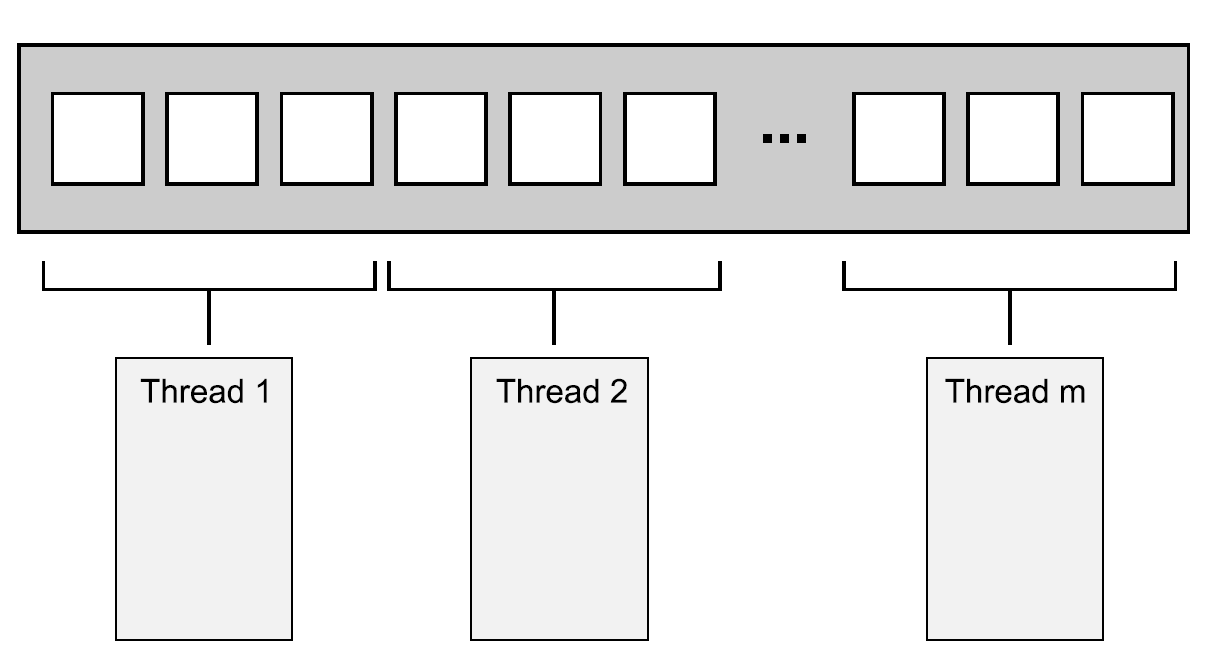
\includegraphics[width=0.7\textwidth]{content/chapter08/images/8-1.png}\\
  图8.1 向线程分发连续的数据块
\end{center}

使用过\textit{MPI}(Message Passing Interface)\footnote[1]{http://www.mpi-forum.org/}和OpenMP\footnote[2]{http://www.openmp.org/}的同学对这个结构一定很熟悉:一项任务被分割成多个,放入一个并行任务集中,执行线程独立的执行这些任务,结果在主线程中合并。这种方式在2.4节中的accumulate的例子中使用过,所有并行任务和主线程的任务都是累加和。对于for\_each来说,主线程将无事可做,因为这个计算不需要处理最终结果。

最后一步对于并行程序来说十分重要,(如代码2.8中的实现)最后一步就是串行的。不过,这一步同样也是能并行化。accumulate实际上是一个递减操作,所以当线程数量大于一个线程上最小处理项时,可以对accumulate进行递归调用。或者工作线程就像做一个完整的任务一样,对步骤进行递减。

虽然这个技术十分强大,但是并不是哪里都适用。有时不能像之前那样,对任务进行整齐的划分,因为只有对数据进行处理后,才能进行明确的划分。这里的方式特别适用了递归算法,下面就来看看这种特别的方式。

\mySubsubsection{8.1.2}{递归划分}

快速排序有两个最基本的步骤:将数据划分到中枢元素之前或之后,然后对中枢元素之前和之后的两半数组再次进行快速排序。这里不能通过对数据的简单划分达到并行,因为只有在一次排序结束后,才能知道哪些项在中枢元素之前和之后。当要对这种算法进行并行化,很自然的会想到使用递归。每一级的递归都会多次调用quick\_sort函数,因为需要知道哪些元素在中枢元素之前和之后。递归调用是完全独立的,因为其访问的是不同的数据集,并且每次迭代都能并发执行。图8.2展示了这样的递归划分。

% ![](../../images/chapter8/8-2.png)
\begin{center}
  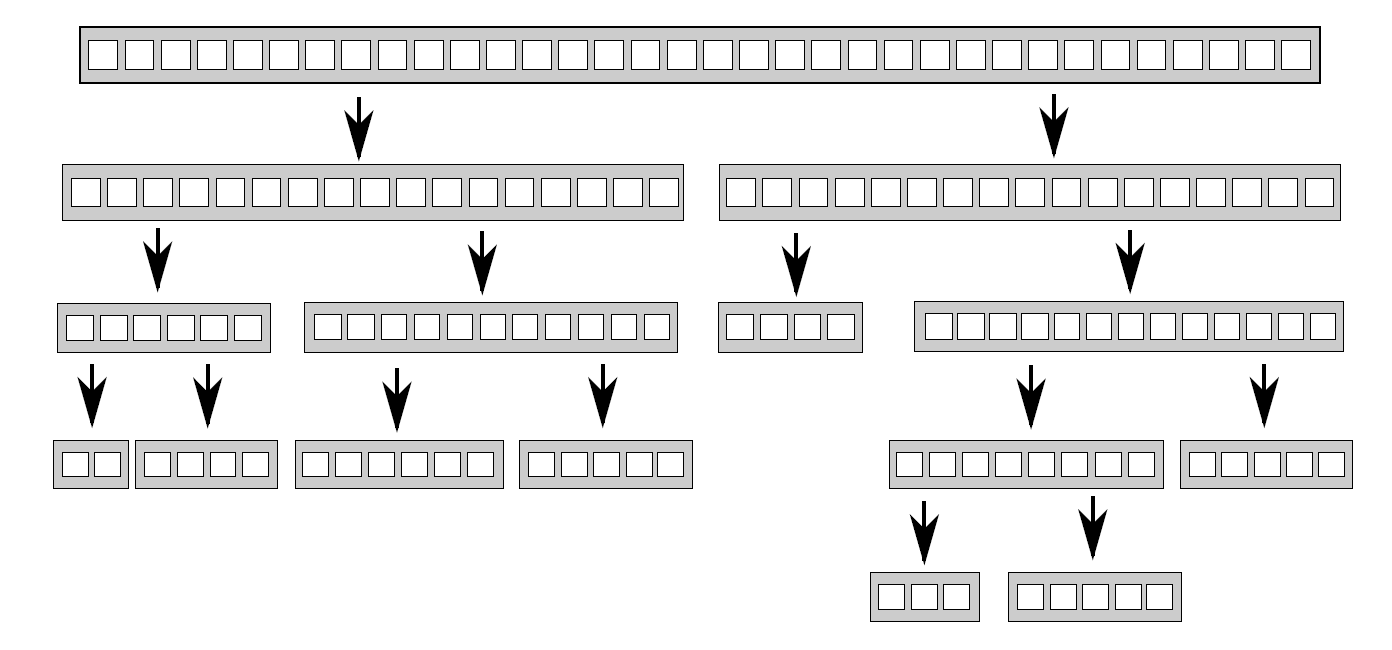
\includegraphics[width=0.7\textwidth]{content/chapter08/images/8-2.png}\\
  图 8.2 递归划分数据
\end{center}

第4章中已经见过这种实现,比起对数据块递归调用函数,使用\texttt{std::async()}可以为每一级生成小于数据块的异步任务。使用\texttt{std::async()}时,C++线程库就能决定何时让一个新线程执行任务,并对任务进行同步。

对一个很大的数据集进行排序时,每层递归都产生新线程,最后就会产生大量的线程。大量线程会对性能有影响,如果线程太多,应用将会运行的很慢。如果数据集过于庞大,会将资源耗尽。所以在递归的基础上进行任务的划分,就是一个不错的主意。只需要将一定数量的数据打包后,交给线程即可。\texttt{std::async()}可以处理这种简单的情况,当然也有其他组选择。

另一种选择是使用\texttt{std::thread::hardware\_concurrency()}函数来确定线程的数量,就像代码2.8中的accumulate()一样。将已排序的数据推到线程安全的栈上(如第6、7章中提及的栈)。线程无所事事时,不是已经完成对自己数据块的梳理,就是在等待一组排序数据的产生。所以,线程可以从栈上获取这组数据,并且对其排序。

下面的代码就是使用以上方式实现。与大多数示例一样,只是演示,而非工业代码。如果编译器支持C++17,最好使用标准库提供的并行算法,这些会在第10章再来讨论。

代码8.1 使用栈的并行快速排序算法——等待数据块排序

\begin{cpp}
template<typename T>
struct sorter  // 1
{
  struct chunk_to_sort
  {
    std::list<T> data;
    std::promise<std::list<T> > promise;
  };

  thread_safe_stack<chunk_to_sort> chunks;  // 2
  std::vector<std::thread> threads;  // 3
  unsigned const max_thread_count;
  std::atomic<bool> end_of_data;

  sorter():
    max_thread_count(std::thread::hardware_concurrency()-1),
    end_of_data(false)
  {}

  ~sorter()  // 4
  {
    end_of_data=true;  // 5

    for(unsigned i=0;i<threads.size();++i)
    {
      threads[i].join();  // 6
    }
  }

  void try_sort_chunk()
  {
    boost::shared_ptr<chunk_to_sort > chunk=chunks.pop();  // 7
    if(chunk)
    {
      sort_chunk(chunk);  // 8
    }
  }

  std::list<T> do_sort(std::list<T>& chunk_data)  // 9
  {
    if(chunk_data.empty())
    {
      return chunk_data;
    }

    std::list<T> result;
    result.splice(result.begin(),chunk_data,chunk_data.begin());
    T const& partition_val=*result.begin();

    typename std::list<T>::iterator divide_point=  // 10
       std::partition(chunk_data.begin(),chunk_data.end(),
        [&](T const& val){return val<partition_val;});

    chunk_to_sort new_lower_chunk;
    new_lower_chunk.data.splice(new_lower_chunk.data.end(),
       chunk_data,chunk_data.begin(),
       divide_point);

    std::future<std::list<T> > new_lower=
      new_lower_chunk.promise.get_future();
    chunks.push(std::move(new_lower_chunk));  // 11
    if(threads.size()<max_thread_count)  // 12
    {
      threads.push_back(std::thread(&sorter<T>::sort_thread,this));
    }

    std::list<T> new_higher(do_sort(chunk_data));

    result.splice(result.end(),new_higher);
    while(new_lower.wait_for(std::chrono::seconds(0)) !=
       std::future_status::ready)  // 13
    {
      try_sort_chunk();  // 14
    }

    result.splice(result.begin(),new_lower.get());
    return result;
  }

  void sort_chunk(boost::shared_ptr<chunk_to_sort> const& chunk)
  {
    chunk->promise.set_value(do_sort(chunk->data));  // 15
  }

  void sort_thread()
  {
    while(!end_of_data)  // 16
    {
      try_sort_chunk();  // 17
      std::this_thread::yield();  // 18
    }
  }
};

template<typename T>
std::list<T> parallel_quick_sort(std::list<T> input)  // 19
{
  if(input.empty())
  {
    return input;
  }
  sorter<T> s;

  return s.do_sort(input);  // 20
}
\end{cpp}

parallel\_quick\_sort函数⑲代表了sorter类①的功能,支持在栈上简单的存储无序数据块②,并且对线程进行设置③。do\_sort成员函数⑨主要是对数据进行划分⑩。相较于对每个数据块产生新线程,这次会将数据块推到栈上⑪,并使用备用处理器⑫产生新线程。因为小于部分的数据块可能由其他线程进行处理,就需要等待线程完成⑬。为了让所有事情顺利进行(只有一个线程和其他所有线程都忙碌时),线程处于等待状态时⑭,就让当前线程尝试处理栈上的数据。try\_sort\_chunk只是从栈上弹出一个数据块⑦,并且对其进行排序⑧,将结果存在promise中,让线程对已存在于栈上的数据块进行提取⑮。

当没有设置end\_of\_data时⑯,新生成的线程还在尝试从栈上获取需要排序的数据块⑰。循环检查中,也要给其他线程机会⑱,可以从栈上取下数据块进行操作。这里的实现依赖于sorter类④对线程的清理。当所有数据都已完成排序,do\_sort将会返回(即使还有工作线程在运行),所以主线程将会从parallel\_quick\_sort⑳中返回,之后会销毁sorter对象。析构函数会设置end\_of\_data标志⑤,以及等待所有线程完成工作⑥,标志将决定是否终止线程函数的内部循环⑯。

这个方案中,不用为spawn\_task产生的无数线程所困扰,也不用再依赖C++线程库,这里可以选择执行线程的数量。该方案的线程数量就是\texttt{std::thread::hardware\_concurrency()},这样就能避免任务过于频繁的切换。不过,这里还有两个问题:线程管理和通讯。要解决这两个问题就要增加代码的复杂度,虽然线程对数据项分开处理,不过所有对栈的访问都可以向栈添加新的数据块,并且移出数据块以作处理。重度竞争会降低性能,原因会在后面给出。

这个方案使用到了特殊的线程池——所有线程任务都来源于一个等待链表,然后线程会去完成任务,任务完成后会再来链表提取任务。这个线程池会出问题(包括对工作链表的竞争),问题的解决方案将在第9章提到。关于多处理器的问题,将会在本章后面的章节中做出更为详细的介绍(详见8.2.1)。

任务几种划分方法:处理前划分和递归划分(都需要事先知道数据的长度固定),还有上面的划分方式。事情并非总是这样好解决,当数据是动态生成或是通过外部输入,那这里的办法就不适用了。这种情况下,基于任务类型的划分方式,就要好于基于数据的划分方式。

\mySubsubsection{8.1.3}{通过任务类型划分}

虽然会为每个线程分配不同的数据块,因为这里每个线程对每个数据块的操作是相同的,所以工作的划分(无论是之前就划分好,还是使用递归的方式划分)仍停留在理论阶段。另一种选择是让线程做专门的工作,就是每个线程做不同的工作,就像水管工和电工在建造一所屋子的时候,所做的不同工作那样。线程可能会对同一段数据进行操作,但对数据进行不同的操作。

对分工的排序,也就是分离关注点。每个线程都有不同的任务,这意味着真正意义上的线程独立。其他线程偶尔会向特定线程交付数据,或是通过触发事件的方式来进行处理。不过总体而言,每个线程只需要关注自己所要做的事情即可。其本身就是良好的设计,每一段代码只对自己的部分负责。

\textbf{分离关注}

当有多个任务需要持续运行一段时间,或需要及时进行处理的事件(比如,按键事件或传入网络数据),且还有其他任务正在运行时,单线程应用采用的是单责任原则处理冲突。单线程中代码会执行任务A(部分)后,再去执行任务B(部分),再检查按钮事件,再检查传入的网络包,然后在循环回去,执行任务A。这将会使得任务A复杂化,因为需要存储完成状态,以及定期从主循环中返回。如果在循环中添加了很多任务,那么程序将运行的很慢。并且用户会发现,在按下按键后,很久之后才会有反应。我确定你已经在一些程序中见过这种情况:给程序分配一项任务后,发现接口会封锁,直到这项任务完成。

当使用独立线程执行任务时,操作系统会帮忙处理接口问题。执行任务A时,线程可以专注于执行任务,而不用为保存状态从主循环中返回。操作系统会自动保存状态,当需要的时候将线程切换到任务B或任务C。如果目标系统是带有多核或多处理器,任务A和任务B可很可能真正的并发执行。处理按键时间或网络包的代码,就能及时执行了。所有事情都完成的很好,用户得到了及时的响应。当然,作为开发者只需要写具体操作的代码即可,不用将控制分支和用户交互混在一起了。

听起来不错,玫瑰色的愿景呀。事实真会如上面所说的那样简单?一切取决于细节。如果每件事都是独立的,线程间就不需要交互,这样的话一切都很简单。不幸的是,现实没那么美好。后台那些优雅的任务,经常会被用户要求做一些事情,并且它们需要通过更新用户接口的方式,来让用户知道它们完成了任务。或者,用户可能想要取消任务,就需要用户向接口发送一条消息,告知后台任务停止运行。这两种情况都需要认真考虑、设计、以及适当的同步,不过这里还是会对分离的部分产生担心。用户接口线程只能处理用户接口,当其他线程告诉该线程要做什么时,用户接口线程会进行更新。同样,后台线程只运行它们所关注的任务,有时会发生“允许任务被其他线程所停止”的情况。这两种情况下,后台线程需要照顾来自其他线程的请求,线程本身只知道它们的请求与自己的任务有所关联。

多线程下有两个危险需要分离。第一个是对错误的担忧(主要表现为线程间共享着很多的数据),第二是不同的线程要相互等待,这两种情况都是因为线程间很密切的交互。这种情况发生时,就需要看一下为什么需要这么多交互。当所有交互都有同样的问题,就应该使用单线程来解决,并将引用同一源的线程提取出来。或者当有两个线程需要频繁的交流,在没有其他线程时,就可以将这两个线程合为一个线程。

当通过任务类型对线程间的任务进行划分时,不应该让线程处于隔离态。当多个输入数据集需要使用同样的操作序列,可以将序列中的操作分成多个阶段让线程执行。

\textbf{划分任务序列}

当任务会应用到相同操作序列,去处理独立的数据项时,就可以使用\textit{流水线}(pipeline)系统进行并发。这好比一个物理管道:数据流从管道一端进入,进行一系列操作后,从管道另一端出去。

使用这种方式划分工作,可以为流水线中的每一阶段操作创建一个独立线程。当一个操作完成,数据元素会放在队列中,供下一阶段的线程使用。这就允许第一个线程在完成对于第一个数据块的操作时,第二个线程可以对第一个数据块执行管线中的第二个操作。

这就是线程间划分数据的一种替代方案(如8.1.1描述),这种方式适合于操作开始前,且对输入数据处长度不清楚的情况。例如:数据来源可能是从网络,或者可能是通过扫描文件系统来确定要处理的文件。

流水线对于队列中的耗时操作处理也很合理,通过对线程间任务的划分,就能对应用的性能有所改善。假设有20个数据项,需要在四核的机器上处理,并且每一个数据项需要四个步骤来完成操作,每一步都需要3秒来完成。如果将数据分给了四个线程,每个线程上就有5个数据项要处理。假设在处理时,没有其他线程对处理过程进行影响,在12秒后4个数据项处理完成,24秒后8个数据项处理完成,以此类推。当20个数据项都完成操作,就需要1分钟的时间。管线中就会完全不同,四步可以交给四个内核,第一个数据项可以被每一个核进行处理,所以其还是会消耗12秒。在12秒后你就能得到一个处理过的数据项,这相较于数据划分并没有好多少。不过,当流水线动起来,事情就会不一样了。第一个核处理第一个数据项后,数据项就会交给下一个内核,所以第一个核在处理完第一个数据项后,其还可以对第二个数据项进行处理。在12秒后,每3秒将会得到一个已处理的数据项,这就要好于每隔12秒完成4个数据项。

为什么整批处理的时间要长于流水线呢?因为最后一个核在开始处理第一个元素时,等待了9秒。更平滑的操作能在某些情况下获益更多,考虑如下情况:当一个系统用来播放高清数字视频。为了让视频能够播放,至少要保证25帧每秒的解码速度。这些图像需要有均匀的间隔,才会给观众留有连续播放的感觉。一个应用可以在1秒解码100帧,不过在解完就需要暂停1s的时候,这个应用就没有意义了。另一方面,观众能接受在视频开始播放的时候有一定的延迟。这种情况,并行使用流水线就能得到稳定的解码率。

看了这么多线程间划分工作的技术,接下来让我们来看一下在多线程系统中有哪些因素会影响性能,并了解一下这些因素是如何影响划分方案的。

% ----------

% [1] http://www.mpi-forum.org/

% [2] http://www.openmp.org/
